% !TeX spellcheck = en_US
%%%%  Las secciones de texto con fórmulas se separan con %%%%
%% Las fórmulas presentes entre 2 secciones de texto se separan con %%

%%%%%%%%%%%%%%%
%%  Capítulo 1: Introducción  %%
%%%%%%%%%%%%%%%

%%%%
\section{Reseña histórica}
\label{sec_intro_resenia}
%%%%

%%%%
Las bases de la teoría electromagnética clásica para el dominio macroscópico fueron formuladas por James Clerk Maxwell en 1873, en base al conocimiento previo desarrollado por Gauss, Ampère y Faraday, entre otros. Entre 1885 y 1887, Oliver Heaviside simplificó las expresiones e introdujo la notación vectorial actual, facilitando así el modelado de guías de ondas y líneas de transmisión \cite{Pozar:MwEngineering}.

En base a estos trabajos, Heinrich Hertz diseñó, entre 1887 y 1891, una serie de experimentos que validaron la teoría de ondas electromagnéticas propuesta por Maxwell. En 1886, Hertz construyó la primer antena dipolo, y en 1888, la primer antena parabólica, alimentada por un dipolo de 450 MHz, dando el puntapié inicial para el desarrollo de la radio durante la primera mitad del siglo \textsc{XX}.

El primer análisis de la propagación de ondas electromagnéticas en guías de ondas metálicas, publicado por Lord Rayleigh en 1897, y el posterior estudio teórico del comportamiento de ondas en guías dieléctricas por Debye y Hondros, en 1910, sentaron los cimientos para que durante la década del '30 comenzaran trabajos experimentales en transporte de ondas electromagnéticas en los laboratorios Bell \cite{Collin:GuidedWaves}.

Los conjuntos de antenas se popularizaron a partir de la aparición de la antena de Yagui-Uda en 1926, formada por elementos lineales que dan lugar a una fase fija. Recién durante la Segunda Guerra Mundial surgieron los conjuntos de antena de fase variable \cite{Stutzman:AntennaTheory}, y las guías de ondas y las antenas tomaron un lugar prioritario entre los ingenieros, matemáticos y físicos de la época, lo que permitió el desarrollo de métodos de análisis para facilitar la formulación de problemas con condiciones de borde complejas.

Recién finalizada la Segunda Guerra Mundial se comenzaron a fabricar circuitos \textit{microstrip}. En 1953, G. A. Deschamps presentó el primer trabajo sobre antenas con la misma tecnología, y la primer patente en ese sentido se registró en 1955 \cite{Balanis:Handbook}. Aún así, recién en la década del '70 comenzaron a utilizarse en aplicaciones prácticas, principalmente debido a la aparición de sustratos con bajas tangentes de pérdida, la mejora en técnicas de fotolitografía, y la optimización de modelos teóricos \cite{Barthia:Handbook}, que permitieron solucionar los problemas de dispersión y aparición de modos indeseados. Sin embargo, la simplificación constructiva trajo aparejados problemas de acoplamiento mutuo, que debieron ser abordados por técnicas de filtrado y blindaje.

%%%%
% NO QUEDÓ BIEN COMPLETO.
%%%%
\section{Ecuaciones de Maxwell}
\label{subsec_ecuaciones_maxwell}
%%%%
La teoría electromagnética propuesta por Maxwell, y simplificada por Heaviside, se reduce a cuatro ecuaciones diferenciales lineales vectoriales e interdependientes que, en notación diferencial, quedan expresadas como se observa a la izquierda de la ecuación \ref{eq:Maxwell} \cite{Pozar:MwEngineering}:

\begin{align}
\label{eq:Maxwell}
\left.\begin{array}{rr@{\mskip\thickmuskip}l}
\text{Faraday} &\nabla \times \vec{E} & = -\frac{\partial \vec{B}}{\partial t} - \vec{M}\\
\text{Ampère} &\nabla \times \vec{H} & = \frac{\partial \vec{D}}{\partial t} + \vec{J} \\
\text{Gauss} &\nabla \cdot \vec{D} & = \rho \\
& \nabla \cdot \vec{B} & = 0
\end{array} \right\}
\quad \implies \quad
\left\{\begin{array}{r@{\mskip\thickmuskip}l}
\nabla \times \vec{E} & = -j \omega \vec{B} - \vec{M} \\
\nabla \times \vec{H} & = j \omega \vec{D} + \vec{J} \\
\nabla \cdot \vec{D} & = \rho\\
\nabla \cdot \vec{B} & = 0
\end{array}\right.
\end{align}

donde $\vec{E}$ es el campo eléctrico, en $(V/m)$; $\vec{H}$ es el campo magnético, en $(A/m)$; $\vec{D}$ es la densidad de flujo eléctrico, en $(C/m^2)$; $\vec{B}$ es la densidad de flujo magnético, en $(Wb/m)$; $\vec{M}$ es la densidad de corriente magnética, en $(V/m)$, y se considera por completitud y simetría; $\vec{J}$ es la densidad de corriente eléctrica, en $(A/m^2)$; y $\rho$ es la densidad de carga eléctrica, en $(C/m^2)$.

De las ecuaciones \ref{eq:Maxwell} se deduce que las fuentes de campo electromagnético son las corrientes $\vec{M}$ y $\vec{J}$, y la densidad de carga eléctrica $\rho$.

Aplicando la divergencia a la ecuación de Ampere, y recordando que $\nabla \cdot (\nabla \times F) = 0$, se obtiene la ecuación de continuidad, que representa la conservación de la carga, o la continuidad de la corriente.

\begin{equation}
	\label{eq:continuidad}
	\nabla \cdot \vec{J} + \frac{\partial \rho}{\partial t} = 0
\end{equation}
%%%%

Dado que la mayor parte del análisis se realiza sobre campos de comportamiento armónico y en régimen permanente, la dependencia del tiempo de la ecuaciones de Maxwell se suele simplificar, y se puede utilizar notación fasorial. Para esto, todos los campos se consideran complejos, y la dependencia temporal, $e^{j \omega t}$, se suele dejar implícita, dado que resulta común para todos los términos. Considerando que cualquier variación en el tiempo físicamente realizable puede ser descompuesta según la transformada de Fourier, no hay pérdida de generalidad al tratar a las ecuaciones de Maxwell de esta manera. Así, las derivadas respecto del tiempo resultan más sencillas, y los vectores de campos se vuelven funciones vectoriales complejas dependientes sólo de coordenadas espaciales \cite{Collin:GuidedWaves}. El resultado de esta simplificación se observa en el lado derecho de la ecuación \ref{eq:Maxwell}.

\subsection{Campos en medios materiales}
\label{subsec_campos_en_dielectricos}

Un campo eléctrico aplicado sobre cualquier material dieléctrico genera una polarización de sus átomos y/o moléculas, creando momentos dipolares eléctricos (o alineándolos, si en el material existían previamente), y dando lugar a un vector de polarización adicional, $\vec{P}_e$, que genera un decrecimiento en el campo eléctrico presente en el material. En el mismo sentido, un campo magnético aplicado sobre un medio material podría ser capaz de alinear los momentos dipolares magnéticos en un material magnético, produciendo un vector de polarización magnética $P_m$. Si el medio es, además, lineal e isotrópico, dichas polarizaciones son proporcionales al campo aplicado, de forma que $\vec{P}_e = \epsilon_0 \chi_e \vec{E}$ y $\vec{P}_m = \chi_m \vec{H}$, con $\chi_e$ y $\chi_m$ las susceptibilidades eléctrica y magnética, respectivamente. Dado que las susceptibilidades toman valores complejos, los medios materiales poseen permitividades eléctricas y permeabilidades magnéticas también complejas, asociadas a las pérdidas debidas al amortiguamiento causado por los momentos dipolares respectivos \cite{Fernandez:Electromag}. Las relaciones constitutivas resultan, entonces:
\begin{subequations}
	\label{eq:polarization_vector}
	\begin{align}
		\vec{D} = \epsilon_0 \vec{E} + \vec{P}_e = \epsilon_0 (1+\chi_e)\vec{E} = \epsilon \vec{E} &= (\epsilon' - j \epsilon'') \vec{E}\\
		\vec{B} = \mu_0 (\vec{H} + \vec{P}_m) = \mu_0 (1+\chi_m)\vec{H} = \mu \vec{H} &= (\mu' - j \mu'') \vec{H}
	\end{align}
\end{subequations}

Si, además, el material posee una conductividad $\sigma$, la aplicación de un campo eléctrico da lugar a la aparición de una densidad de corriente $\vec{J}$, que en algunos casos, cuando $\sigma$ es independiente del campo eléctrico aplicado, de la dirección del mismo y de la posición, se puede expresar según la ley de Ohm:

\begin{equation}
	\label{eq:ohms_law}
	\vec{J} = \sigma \vec{E}
\end{equation}

La ecuación de Ampère de \ref{eq:Maxwell} queda, entonces, expresada como
\begin{subequations}
	\begin{align}
		\nabla \times \vec{H} & = j \omega \vec{D} + \vec{J} = j \omega \epsilon \vec{E} + \sigma \vec{E} = j \omega \epsilon' \vec{E} + (\omega \epsilon'' + \sigma)\vec{E}\\
		& = j \omega \left( \epsilon' - j\epsilon'' - j \frac{\sigma}{\omega} \right) \vec{E}
	\end{align}
\end{subequations}

La relación entre la parte imaginaria y la parte real de la corriente total de desplazamiento se conoce como tangente de pérdidas \cite{Pozar:MwEngineering}:

\begin{equation}
	tan \; \delta = \frac{\omega \epsilon'' + \sigma}{\omega \epsilon'}
\end{equation}

Cuando el material no es homogéneo, los coeficientes $\epsilon$ y $\mu$ dependen de la posición. Si, además, el material es anisotrópico, como en el caso de los cristales y gases ionizados, la relaciones expresadas antes entre los vectores de polarizacón ($\vec{P}_e$ y $\vec{P}_m$)y los campos no se cumplen, sino que deben ser expresadas como tensores de rango 2 (diadas), como se muestra en la ecuación \ref{eq:diadas}, explicitando así su dependencia de la dirección \cite{Collin:GuidedWaves}. Si, además, el material no es lineal, los coeficientes $\epsilon_{ij}$ y $\mu_{ij}$ pueden ser funciones de $\vec{E}$ y $\vec{H}$ respectivamente.

\begin{equation} \label{eq:diadas}
\begin{bmatrix}
D_x \\
D_y \\
D_z
\end{bmatrix}
=
\begin{bmatrix}
\epsilon_{xx} & \epsilon_{xy} & \epsilon_{xz} \\
\epsilon_{yx} & \epsilon_{yy} & \epsilon_{yz} \\
\epsilon_{zx} & \epsilon_{zy} & \epsilon_{zz}
\end{bmatrix}
\begin{bmatrix}
E_x \\
E_y \\
E_z
\end{bmatrix}
\qquad\text{y}\qquad
\begin{bmatrix}
B_x \\
B_y \\
B_z
\end{bmatrix}
=
\begin{bmatrix}
\mu_{xx} & \mu_{xy} & \mu_{xz} \\
\mu_{yx} & \mu_{yy} & \mu_{yz} \\
\mu_{zx} & \mu_{zy} & \mu_{zz}
\end{bmatrix}
\begin{bmatrix}
H_x \\
H_y \\
H_z
\end{bmatrix}
\end{equation}

\subsection{Condiciones de borde} \label{sec:condiciones-borde}

\begin{figure}[htp]
	\centering
	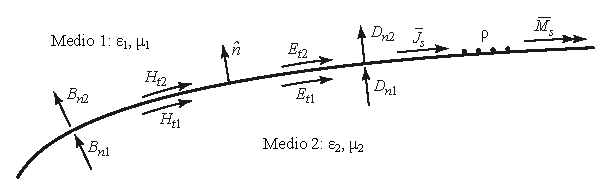
\includegraphics[width=0.8\textwidth]{intro_electro/condiciones_borde.eps}
	\caption{Corrientes, campos y carga superficial en una interfaz general entre dos medios \cite{Pozar:MwEngineering}}
	\label{fig:condiciones_borde}
\end{figure}

Si se considera una interfaz entre dos medios, como la que se muestra en la figura \ref{fig:condiciones_borde}, a partir de las ecuaciones de Maxwell y los teoremas integrales, se pueden deducir las siguientes condiciones de borde:
\begin{subequations}
	\label{eq:condiciones_borde}
	\begin{align}
		\hat{n} \cdot (\vec{D}_{2} - \vec{D}_{1}) & = \rho_s \\
		\hat{n} \cdot (\vec{B}_{2} - \vec{B}_{2}) & = 0 \\
		\hat{n} \times (\vec{E}_2 - \vec{E}_1)  & = - \vec{M}_s \\
		\hat{n} \times (\vec{H}_2 - \vec{H}_1) & = \vec{J}_s
	\end{align}
\end{subequations}

\subsubsection{Campos sobre una superficie dieléctrica}
Dado que en una interfaz entre dos dieléctricos no hay carga eléctrica ni densidades de corriente, las ecuaciones \ref{eq:condiciones_borde} establecen que \textbf{las componentes normales de los vectores $\vec{D}$ y $\vec{B}$ se conservan, y que las componentes tangenciales de $\vec{E}$ y $\vec{H}$ también lo hacen}.

\subsubsection{Campos sobre una superficie conductora eléctrica}
Si el conductor no tiene pérdidas ($\sigma \rightarrow \infty$), todos los campos deben ser cero en su interior, dado que la profundidad de penetración se anula. Considerando, además, que $\vec{M}_s = 0$, la componente tangencial del campo eléctrico, \textbf{$E_t$ desaparece sobre la superficie del conductor}. Dado que la diferencia entre las componentes normales del campo magnético está dada por $\vec{J}_s$, y el campo magnético debe anularse en el conductor, \textbf{la densidad de corriente superficial está dada únicamente por el campo magnético externo al conductor}. En el mismo sentido, la densidad de carga superficial $\rho_s$ es la expresión, sobre la superficie del conductor, de la componente normal de $\vec{D}$.

% SKIN DEPTH

\subsubsection{Campos sobre una superficie conductora magnética}
Dado que la superficie conductora magnética representa el caso dual al de la superficie conductora eléctrica, en este caso se espera que la \textbf{componente tangencial de $\vec{H}$ se anule sobre la superficie}, mientras que la componente tangencial del campo eléctrico dé lugar a corrientes magnéticas sobre la misma.

%%%%% QUEDA DECRI QUE PASA CON UNA CORRIWENTE EN HORIZRAON O VERTICAL - LIBRO DE YAMAT, PAG 10.
%% COMPLETAR CON COLLIN %%

\section{Ecuación de onda}
\label{subsec_eq_de_onda}
%%%%

Al considerar una región del espacio lineal, isotrópica y homogénea, se puede calcular el rotor de la primera ecuación de Maxwell, aplicar la segunda ecuación y, recordando que $\nabla \times \nabla \times \vec{E} = \nabla \nabla \cdot \vec{E} - \nabla^2\vec{E}$, donde $\nabla \cdot \vec{E} = \rho/\epsilon$, se puede deducir que:

\begin{align}
	\nabla \times \nabla \times \vec{E} & = -j \omega \mu \nabla \times \vec{H} - \nabla \times \vec{M} \notag \\
	\nabla \nabla \cdot \vec{E} - \nabla^2 \vec{E} & = -j \omega \mu \nabla \times \vec{H} - \nabla \times \vec{M} \notag \\
	\frac{\nabla \rho}{\epsilon} - \nabla^2 \vec{E} & = \omega^2 \mu \epsilon \vec{E} - j \omega \mu \vec{J} - \nabla \times \vec{M} \notag\\
	\nabla^2 \vec{E} + \omega^2 \mu \epsilon \vec{E} & = j \omega \mu \vec{J} + \frac{\nabla \rho}{\epsilon} + \nabla \times \vec{M}
	\label{eq:eq_ondas_completa_E}
\end{align}

en el mismo sentido, para el campo magnético:
\begin{align}
	\nabla \times \nabla \times \vec{H} & = j \omega \nabla \times \vec{D} +  \nabla \times \vec{J} \notag \\
	\nabla \nabla \cdot \vec{H} - \nabla^2 \vec{H} & = j \omega \epsilon \nabla \times \vec{E} + \nabla \times \vec{J} \notag \\
	\frac{1}{\mu} \nabla (\cancelto{0}{\nabla \cdot \vec{B}}) - \nabla^2 \vec{H} & = j \omega \epsilon (-j \omega \vec{B} - \vec{M}) + \nabla \times \vec{J} \notag \\
	\nabla^2 \vec{H} + \omega^2 \epsilon \mu \vec{H} & =  j \omega \epsilon \vec{M} - \nabla \times \vec{J}
	\label{eq:eq_ondas_completa_H}
\end{align}

De las ecuaciones anteriores se observa que el campo magnético está determinado por la componente rotacional de la corriente eléctrica, mientras que el campo eléctrico está determinado por todas las componentes de la misma. De manera análoga, se cumple la relación inversa para el caso de la corriente magnética.

Si, además, la región del espacio es libre de fuentes, se deducen las ecuaciones de Helmholtz para ambos campos, donde $k$ es la constante de propagación o número de onda, en unidades de $(1/m)$:

\begin{subequations}
	\label{eq:Helmholtz}
	\begin{align}
		\nabla \times \vec{E} + k^2 \vec{E} = 0 \label{eq:Helmholtz_E} \\
		\nabla \times \vec{H} + k^2 \vec{H} = 0 \label{eq:Helmholtz_H}
	\end{align}
\end{subequations}
%%%%

Para el caso sin pérdidas se puede expresar como $k = \omega \sqrt{\mu \epsilon}$, mientras que \textbf{si se considera que existen pérdidas óhmicas, las mismas pueden ser tenidas en cuenta si $k$ asume el valor complejo} $-j\gamma$, con $\gamma = j\alpha + \beta = j \omega \sqrt{\mu \epsilon} \sqrt{1-j \sigma/(\omega \epsilon)}$. Para el caso de un buen conductor, $\gamma = j\alpha + \beta = j \omega \sqrt{\mu \epsilon} \sqrt{\sigma/(\omega \epsilon)} = (1+j) \sqrt{\omega \mu \sigma/2}$, lo que nos permite definir la \textbf{profundidad de penetración} como $\delta_s = 1/\alpha = \sqrt{2/(\omega \mu \sigma)}$, que decrece con la frecuencia.

En coordenadas cartesianas, la ecuación \ref{eq:Helmholtz_E} se puede escribir como indica la ecuación \ref{eq:Helmholtz_cartesianas_completo}, que además se cumple para todas las coordenadas en que se desarrolla el campo $\vec{E}$. Para cada una de estas coordenadas, resulta sencillo aplicar el método de separación de variables, de forma que $E_i = f(x)g(y)h(z)$ para $i=x, y,$ ó $z$, donde las funciones $f(x)$, $g(y)$ y $h(z)$ son independientes.

\begin{equation}
	\label{eq:Helmholtz_cartesianas_completo}
	\nabla^2 \vec{E} + k_0^2 \vec{E} = \frac{\partial^2 \vec{E}}{\partial x^2} + \frac{\partial^2 \vec{E}}{\partial y^2} + \frac{\partial^2 \vec{E}}{\partial z^2} +  k_0^2 \vec{E} = 0
\end{equation}

Sustituyendo, para la ecuación de Helmholtz de cada coordenada, la expresión de $E_i$, se obtiene que $\frac{f''(x)}{f(x)} + \frac{g''(y)}{g(y)} + \frac{h''(z)}{h(z)} + k_0^2 = 0$, y dado que las funciones propuestas son independientes, cada uno de los términos de la ecuación anterior deben dar lugar a una constante, de modo que $\frac{f''(x)}{f(x)} = -k_x^2$, $\frac{g''(y)}{g(y)} = -k_y^2$ y $\frac{h''(z)}{h(z)} = -k_z^2$. Esto nos permite concluir que:

\begin{equation}
	\label{eq:numero_de_onda}
	k_x^2 + k_y^2 + k_z^2 = k_0^2 \\
\end{equation}

Quedan, entonces, tres ecuaciones diferenciales ordinarias:

\begin{equation}
	\frac{d^2 f}{dx^2} + k_x^2 f = 0; \qquad \frac{d^2 g}{dy^2} + k_y^2 g = 0; \qquad \frac{d^2 h}{dz^2} + k_z^2 h = 0; \nonumber
\end{equation}

cuyas soluciones son de la forma $e^{\pm j k_i i}$, con $i = x, y$ o $z$, respectivamente. Las soluciones con un signo positivo en el exponente corresponden a ondas que viajan en la dirección negativa ($-x, -y, -z$), mientras que las que tienen un signo negativo corresponden a ondas que viajan en la dirección positiva. Dado que ambas soluciones son válidas y posibles, en función de las condiciones de borde, en general la expresión de un campo $E_i (x, y, z), i=x,y,z$ quedará establecida como la suma de ambas, afectadas por un factor de amplitud dependiente de la coordenada evaluada. Para el caso de ondas que viajan en la dirección positiva:

\begin{equation}
	E_i(x,y,z) = A_i \;e^{-j(k_x x + k_y y + k_z z)}, \quad i=x,y,z \nonumber
\end{equation}

Si definimos como $\hat{n}$ al versor en la dirección de propagación, podemos definir el vector de número de onda, $\vec{k}$, como:

\begin{equation}
	\label{eq:vector_numero_de_onda}
	\vec{k} = k_x \hat{x} + k_y \hat{y} + k_z \hat{z} = k_o \hat{n} \nonumber
\end{equation}

De esta forma, se puede expresar, estableciendo $\vec{E}_0 = A \hat{x} + B \hat{y} + C \hat{z}$, y $\vec{r} = x \hat{x} + y \hat{y} + z \hat{z}$, el campo eléctrico como:

\begin{equation}
	\label{eq:electric_field_wave_solution}
	\vec{E} = \vec{E}_0 e^{-j\vec{k} \cdot \vec{r}}
\end{equation}

Para el caso con pérdidas, y considerando que la dirección de propagación es $z$, las componentes $x$ e $y$ se comportan como:

\begin{equation}
E_i(z) = E_i \; e^{-\gamma z} = E_i \; e^{-\alpha z} \; e^{-j \beta z}, \quad i=x,y \nonumber
\end{equation}

Al expresar la divergencia del campo eléctrico de la ecuación \ref{eq:electric_field_wave_solution}, que en una región sin fuentes es nula, y recordando que $\nabla \cdot (f \vec{A}) = \vec{A} \cdot \nabla f + f \nabla \cdot \vec{A}$, se obtiene:


\begin{align}
	\nabla \cdot \vec{E} = \nabla \cdot \vec{E}_0 e^{-j\vec{k} \cdot \vec{r}} & = \vec{E}_0 \cdot \nabla e^{-j \vec{k} \vec{r}} + e^{-j \vec{k} \vec{r}} \cancelto{0}{\nabla \cdot \vec{E}_0} = 0 \nonumber \\
	& = -j \vec{k} \cdot \vec{E}_0 e^{-j \vec{k} \vec{r}} = 0
\end{align}

De lo que se puede deducir que $\vec{k} \cdot \vec{E}_0 = 0$, de modo que el campo eléctrico, en una onda plana, es siempre perpendicular a la dirección de propagación.

De la ecuación de Faraday de \ref{eq:Maxwell}, considerando espacio libre de cargas, se puede deducir que el campo magnético es siempre ortogonal al campo eléctrico y a la dirección de propagación, y que los campos están relacionados de forma que \cite{Fernandez:Electromag}:

\begin{equation}
	\vec{H}(\vec{r},t) = \pm \frac{\hat{n} \times \vec{E}(\vec{r},r)}{\eta}
\end{equation}

donde $\eta$ es la impedancia de onda, que tiene la forma $\eta = j \omega \mu / \gamma$. Para el caso del vacío, la impedancia intrínseca se denota $\eta_0$ y tiene un valor de $377\; \Omega$, mientras que para otros materiales está determinada por su permitividad eléctrica y permeabilidad magnética, y puede ser compleja si hay pérdidas.

La velocidad de fase se define como $v_p=\omega/\beta$, que para el caso sin pérdidas queda como $1/\sqrt{\mu \epsilon}$, y que para el caso particular del vacío, se expresa como $1/\sqrt{\mu_0 \epsilon_0} = c$, donde $c$ es la velocidad de la luz en el vacío. Así, la velocidad de fase en cualquier medio material sin pérdidas resulta $c/\sqrt{\epsilon_r \mu_r}$.

La longitud de onda, $\lambda$, es la distancia espacial entre dos máximos sucesivos, por lo que se expresa como $\lambda = 2\pi / k = v_p/f$.

\subsection{Incidencia de una onda plana sobre una interfaz}

Una onda electromagnética incidente sobre una superficie en un ángulo arbitrario puede analizarse descomponiendo el problema en dos casos canónicos de polarización (dirección del campo eléctrico): perpendicular (TE, trasversal eléctrico) o paralela (TM, transversal magnético) al plano de incidencia, que es el formado por el rayo incidente y la normal a la interfaz. El problema de la incidencia perpendicular a la interfaz combina ambos casos.

\begin{figure} [H]
	\centering 
	\subfigure[Polarización paralela (TM).]{
		\label{fig:oblique_incidence_parallel}
		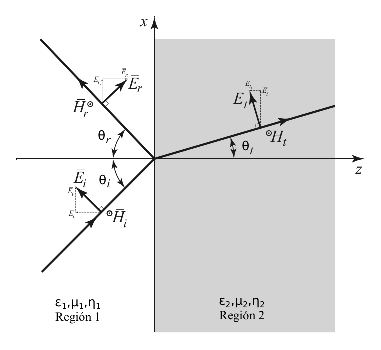
\includegraphics[width=0.45\textwidth]{intro_electro/incidencia_oblicua_paralela-version2.eps}}
	\hspace{5mm}
	\subfigure[Polarización perpendicular (TE).]{
		\label{fig:oblique_incidence_perp}
		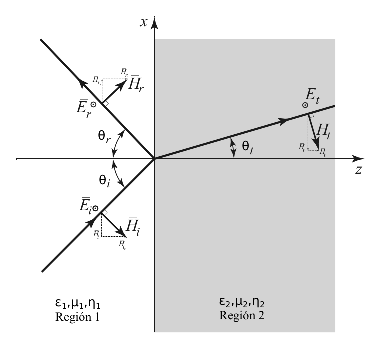
\includegraphics[width=0.45\textwidth]{intro_electro/incidencia_oblicua_perpendicular-version2.eps}}
	\caption{Incidencia oblicua para los dos casos de polarización analizados.}
	\label{fig:oblique_incidence}
\end{figure}

Los campos eléctrico y magnético incidentes, según el sistema de coordenadas definido en la figura \ref{fig:oblique_incidence}, pueden ser expresados, en forma general, como indican las ecuaciones \ref{eq:incident_fields}.

\begin{subequations}
	\label{eq:incident_fields}
	\begin{align}
	\vec{E}_i = \vec{E}_0 \;e^{-j\vec{k}_1 \cdot \vec{r}} \\
	\vec{H}_i = \frac{\hat{k} \times \vec{E}_0}{\eta_1} \;e^{-j\vec{k}_1 \cdot \vec{r}}
	\end{align}
\end{subequations}

donde $\vec{r}=(x,y,z)$, $\vec{k}_1 = \hat{k}_1 \;\omega \sqrt{\mu_1 \epsilon_1}$, $\hat{k}_1$ es la dirección de propagación de la onda plana, y $\eta_1 = \sqrt{\mu_1 / \epsilon_1} = j\omega \mu / \gamma$ es la impedancia de onda de región de incidencia, que puede ser compleja si el medio posee pérdidas.

Se define al coeficiente de reflexión $\Gamma$ como la relación entre la magnitud del campo reflejado y del campo incidente, $E_r / E_i$. De la misma manera, el coeficiente de transmisión $T$ es la relación entre el módulo del campo transmitido al segundo medio y el campo incidente desde el primer medio, $E_t / E_i$, de manera que $1+\Gamma = T$ y que $(1-\Gamma)/\eta_1 = T/\eta_2$. 

Usando estos coeficientes, a partir de las ecuaciones \ref{eq:incident_fields}, y teniendo en cuenta las condiciones de borde descriptas en la sección \ref{sec:condiciones-borde}, se pueden calcular los campos reflejados y transmitidos. Para los dos casos canónicos analizados, los campos incidentes, reflejados y transmitidos se resumen en la tabla \ref{table:incidencia_oblicua}, así como los coeficientes de reflexión y transmisión.

\tabulinesep=1.2mm
\taburulecolor{black!20}
\begin{table}
	
	\begin{tabu} to 1\textwidth {gX[c]@{}X[c]@{}}
		\rowcolor{black!20} & \multicolumn{1}{c}{\textbf{TM}} & \multicolumn{1}{c}{\textbf{TE}}\\
		$\vec{E}_i$
		&
		\scalebox{0.86}{%
			$
			E_0\; (\hat{x}\; \mathrm{cos}\; \theta_i - \hat{z}\; \mathrm{sin}\; \theta_i)\; e^{-j k_1 (x\; \mathrm{sin}\; \theta_i + z\; \mathrm{cos}\; \theta_i)}
			$
		}	
		&
		\scalebox{0.86}{%
			$
			E_0\; \hat{y} \;e^{-j k_1 (x\; \mathrm{sin}\; \theta_i + z\; \mathrm{cos}\; \theta_i)}
			$
		} \\
		$\vec{H}_i$
		&
		\scalebox{0.86}{%
			$
			-\frac{E_0}{\eta_1}\; \hat{y}\; e^{-j k_1 (x\; \mathrm{sin}\; \theta_i + z\; \mathrm{cos}\; \theta_i)}
			$
		}
		&
		\scalebox{0.86}{%
			$
			\frac{E_0}{\eta_1} \;(-\hat{x}\; \mathrm{cos}\; \theta_i + \hat{z}\; \mathrm{sin}\; \theta_i)\; e^{-j k_1 (x\; \mathrm{sin}\; \theta_i + z\; \mathrm{cos}\; \theta_i)}
			$
		} \\
		\hline
	
		$\vec{E}_r$
		&
		\scalebox{0.86}{%
			$
			E_0\; \Gamma\; (\hat{x}\; \mathrm{cos}\; \theta_r + \hat{z}\; \mathrm{sin}\; \theta_r)\; e^{-j k_1 (x\; \mathrm{sin}\; \theta_r - z\; \mathrm{cos}\; \theta_r)}
			$
		}	
		&
		\scalebox{0.86}{%
			$
			E_0\; \Gamma\; \hat{y} \;e^{-j k_1 (x\; \mathrm{sin}\; \theta_r - z\; \mathrm{cos}\; \theta_r)}
			$
		} \\
		$\vec{H}_r$
		&
		\scalebox{0.86}{%
			$
			-\frac{E_0\; \Gamma}{\eta_1}\; \hat{y}\; e^{-j k_1 (x\; \mathrm{sin}\; \theta_r - z\; \mathrm{cos}\; \theta_r)}
			$
		}
		&
		\scalebox{0.86}{%
			$
	 		\frac{E_0\; \Gamma}{\eta_1} \;(\hat{x}\; \mathrm{cos}\; \theta_r + \hat{z}\; \mathrm{sin}\; \theta_r)\; e^{-j k_1 (x\; \mathrm{sin}\; \theta_r - z\; \mathrm{cos}\; \theta_r)}
			$
		} \\
	\hline
		$\vec{E}_t$
		&
		\scalebox{0.86}{%
			$
			E_0\; T\; (\hat{x}\; \mathrm{cos}\; \theta_t - \hat{z}\; \mathrm{sin}\; \theta_t) e^{-j k_2 (x\; \mathrm{sin}\; \theta_t + z\; \mathrm{cos}\; \theta_t)}
			$
		}
		&
		\scalebox{0.86}{%
			$
			E_0\; T\; \hat{y}\; e^{-j k_2 (x\; \mathrm{sin}\; \theta_t + z\; \mathrm{cos}\; \theta_t)}
			$
		} \\
		$\vec{H}_t$
		&
		\scalebox{0.86}{%
			$
	 		\frac{E_0\; T}{\eta_1}\; \hat{y}\; e^{-j k_2 (x\; \mathrm{sin}\; \theta_t + z\; \mathrm{cos}\; \theta_t)}
			$
		}
		&
		\scalebox{0.86}{%
			$
			\frac{E_0\; T}{\eta_2}\; (-\hat{x}\; \mathrm{cos}\; \theta_t + \hat{z}\; \mathrm{sin}\; \theta_t)\; e^{-j k_2 (x\; \mathrm{sin}\; \theta_t + z\; \mathrm{cos}\; \theta_t)}
			$
		} \\
		\hline
		
		$\Gamma$
		&
		$\frac{\eta_2\; cos\; \theta_t - \eta_1 \; cos\; \theta_i}{\eta_2\; cos\; \theta_t + \eta_1 \; cos\; \theta_i}$
		&
		$\frac{\eta_2\; cos\; \theta_i - \eta_1 \; cos\; \theta_t}{\eta_2\; cos\; \theta_i + \eta_1 \; cos\; \theta_t}$
		\\
		$T$
		&
		$\frac{2 \;\eta_2 \; cos\; \theta_i}{\eta_2\; cos\; \theta_t + \eta_1 \; cos\; \theta_i}$
		&
		$\frac{2\; \eta_2 \; cos\; \theta_i}{\eta_2\; cos\; \theta_i + \eta_1 \; cos\; \theta_t}$
	\end{tabu}
	\caption{Campos incidentes, transmitidos y reflejados, y coeficientes de reflexión y transmisión para incidencia oblicua de una onda plana sobre una interfaz dieléctrica}
	\label{table:incidencia_oblicua}
\end{table}

Si se fuerza la continuidad de las componentes tangenciales de los campos sobre la interfaz para ambos casos, $\vec{E}_i^{tg} + \vec{E}_r^{tg} = \vec{E}_t^{tg}$ y $\vec{H}_i^{tg} + \vec{H}_r^{tg} = \vec{H}_t^{tg}$, se obtienen las expresiones \ref{eq:continuidad_campos_paralelo} para el modo TM, y \ref{eq:continuidad_campos_perpendicular} para el modo TE.

\begin{subequations}
	\label{eq:continuidad_campos_paralelo}
	\begin{align}
		cos \; \theta_i \; e^{-j k_1 x sin \; \theta_i} + \Gamma \; cos \; \theta_r \; e^{-j k_1 x \; sin\; \theta_r} &= T\; cos\; \theta_t \; e^{-j k_2 x \; sin\; \theta_t}\\
		\frac{1}{\eta_1} \; e^{-j k_1 x \; sin \theta_i} - \frac{\Gamma}{\eta_1} \; e^{-j k_1 x \; sin \; \theta_r} &= \frac{T}{\eta_2} \; e^{-j k_2 x \; sin\; \theta_t}
	\end{align}
\end{subequations}

\begin{subequations}
	\label{eq:continuidad_campos_perpendicular}
	\begin{align}
	e^{-j k_1 x sin \; \theta_i} + \Gamma \; e^{-j k_1 x \; sin\; \theta_r} &= T\; e^{-j k_2 x \; sin\; \theta_t}\\
	-\frac{1}{\eta_1} cos\; \theta_i \; e^{-j k_1 x \; sin \theta_i} - \frac{\Gamma}{\eta_1} \; cos\; \theta_r e^{-j k_1 x \; sin \; \theta_r} &= -\frac{T}{\eta_2} \; cos\; \theta_t \; e^{-j k_2 x \; sin\; \theta_t}
	\end{align}
\end{subequations}

En estas ecuaciones se observa que a ambos lados de las igualdades, las expresiones son funciones de la posición sobre la interfaz. Para que la condición de borde se cumpla en todos sus puntos, la variación en $x$ debe ser la misma en todos los términos, de forma que el efecto de la variación sea anulado: $k_1 \; sin\; \theta_i = k_1 \; sin \; \theta_r = k_2 \; sin\; \theta_t$.  De esta consideración se deriva la Ley de Snell (asumiendo que $\mu_1 = \mu_2$):

\begin{subequations}
	\label{eq:snell_law}
	\begin{align}
	\theta_i &= \theta_r \\
	k_1 \; sin\; \theta_i = k_2 \; sin\; \theta_t & \overset{\eta=\frac{\omega\mu}{k}}{\Longrightarrow} \eta_2 \; sin\; \theta_i = \eta_1 \; sin\; \theta_t \label{eq:snell_law_second}
	\end{align}
\end{subequations}

Utilizando estas expresiones, y a partir de las ecuaciones \ref{eq:continuidad_campos_paralelo} y \ref{eq:continuidad_campos_perpendicular}, se obtienen las expresiones para los coeficientes de reflexión y transmisión de la tabla \ref{table:incidencia_oblicua}. Resulta importante destacar que, para el caso de incidencia perpendicular ($\theta_i = 0$), los coeficientes quedan simplificados a $\Gamma = (\eta_2 - \eta_1)/(\eta_2 + \eta_1)$ y $T = (2 \; \eta_2)/(\eta_2 + \eta_1)$.

\subsection{Ángulo de Brewster y ángulo crítico}

Se conoce como ángulo de Brewster al ángulo de incidencia $\theta_i$ necesario para que se produzca reflexión nula ($\Gamma = 0$) en una interfaz, cuando sobre ella incide una onda plana en forma oblicua. Este efecto se da únicamente para la polarización TM, es decir, cuando existe componente de campo eléctrico en la dirección normal a la intefaz, por lo que suele ser utilizado como mecanismo para lograr polarización de una onda electromagnética.

Si se anulan los coeficientes de reflexión mostrados en la tabla \ref{table:incidencia_oblicua}, y se utilizan las ecuaciones \ref{eq:snell_law}, se puede observar que en el caso TE se requiere que $sin \; \theta_i / sin \; \theta_t = cos \; \theta_i / cos \; \theta_t = \eta_1 / \eta_2$, lo cual es imposible. Para el caso TM, en cambio, el requisito es $sin \; \theta_i / sin \; \theta_t = cos \; \theta_t / cos \; \theta_i = \eta_1 / \eta_2$, lo cual no supone una contradicción. Multiplicando la ecuación \ref{eq:snell_law_second} y el valor de $\Gamma$ para polarización TM, se obtiene que $sin\;\theta_i \; cos \; \theta_i = sin \; \theta_t \; cos \; \theta_t$, ó $sin \; 2\theta_i = sin \; 2\theta_t$, que se satisface cuando $2\theta_i = \pi - 2\theta_t$, de modo que $\theta_i + \theta_t = \pi/2$. Aplicando esta condición en la Ley de Snell (ecuación \ref{eq:snell_law_second}) se obtiene la expresión del ángulo de Brewster:

\begin{align}
	\label{eq:Brewster_angle}
	tan\;\theta_i^{Brewster} = \frac{\eta_1}{\eta_2}
\end{align}

En ángulo crítico se define como el ángulo de incidencia para el cual la onda incidente es totalmente reflejada, y la onda transmitida no se propagará a la segunda región.

Si se observan las expresiones del coeficiente de transmisión de la tabla \ref{table:incidencia_oblicua}, el único valor de $\theta_i$ para el cual la transmisión es nula es $\pi/2$, es decir, incidencia rasante. Sin embargo, a partir de la ecuación \ref{eq:snell_law_second}, se obtiene que $sin \; \theta_t = \eta_2 / \eta_1\; sin\; \theta_i$. Se puede observar que en los casos en que $\eta_2 > \eta_1$ es posible que el ángulo de transmisión alcance el valor $\pi/2$ antes de que lo haga en ángulo de incidencia. El ángulo crítico, entonces, surge de la expresión:

\begin{equation}
	\label{eq:angulo_critico}
	sin\; \theta_i^c = \frac{\eta_1}{\eta_2}\;\cancelto{1}{sin \; \underbrace{\theta_t}_{\pi/2}} = \sqrt{\frac{\epsilon_2}{\epsilon_1}} \implies \theta_c = arcsin \;\sqrt{\frac{\epsilon_2}{\epsilon_1}} = arcsin \;\frac{\eta_1}{\eta_2}
\end{equation}

Para ángulos mayores a $\theta_c$, las expresiones del coeficiente de reflexión se vuelven complejas y de módulo 1, por lo que toda la energía electromagnética es reflejada, y la onda transmitida tiene un comportamiento evanescente, como se muestra en la figura \ref{fig:angulo_critico}. En la ecuación \ref{eq:angulo_critico} se observa que si $\theta_i > \theta_c$, el ángulo $\theta_t$ pierde significado físico, debido a que $sin\; \theta_t$ debería ser mayor a 1 para cumplir la ecuación.

\begin{figure}[htp]
	\centering
	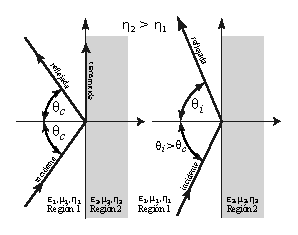
\includegraphics[width=0.5\textwidth]{intro_electro/angulo_critico.eps}
	\caption{Ilustración del comportamiento de una onda plana durante la incidencia con ángulo critico y con ángulo mayor al $\theta_c$.}
	\label{fig:angulo_critico}
\end{figure}

Se debe notar que en el argumento anterior no se consideró la polarización de la onda incidente, por lo que la reflexión completa se puede dar tanto en modo TM como en modo TE, siempre y cuando la incidencia se produzca desde el medio ópticamente más denso al menos denso \cite{Fernandez:Electromag}. Sin embargo, resulta útil expresar el comportamiento de los campos.

Para el caso de una onda incidente con una polarización lineal arbitraria como la expresada en la ecuación \ref{eq:incident_fields}, se debe considerar que la componente longitudinal a la interfaz del vector de onda $\vec{k}$ se mantendrá constante, de modo que ${k_2}_x = {k_1}_x = k_1 \; sin \; \theta_i$. La componente transversal a la interfaz, en cambio, será ${k_2}_z = k_2\; cos \; \theta_t = k_2 \sqrt{1-sin^2\theta_t} = \beta$. Dado que para el caso en que el ángulo incidente es mayor al ángulo crítico se requiere que $sin\;\theta_t > 1$, el valor de ${k_2}_z$ será imaginario, $-i\alpha$. El signo negativo se desprende de la imposibilidad física de un crecimiento exponencial del valor del campo. De esta forma, para direcciones de campos arbitrarias, y teniendo en cuenta el hecho de que el vector $\vec{k}$ se desarrolla sobre el plano de incidencia:

\begin{subequations}
	\begin{align}
		\vec{E}_t (\vec{r},t) = \vec{E}_2 \; e^{-j \vec{k}_2 \cdot \vec{r}} = \vec{E}_2 \; e^{-j({k_2}_x x + {k_2}_z z)} = \vec{E}_2 \; e^{-j(\beta x - j\alpha z)} = \vec{E}_2 \; e^{-j\beta x} \; e^{- \alpha z}\\
		\vec{H}_t (\vec{r},t) = \vec{H}_2 \; e^{-j \vec{k}_2 \cdot \vec{r}} = \vec{H}_2 \; e^{-j({k_2}_x x + {k_2}_z z)} = \vec{H}_2 \; e^{-j(\beta x - j\alpha z)} = \vec{H}_2 \; e^{-j\beta x} \; e^{- \alpha z}
	\end{align}
\end{subequations}

Se observa que en la dirección perpendicular a la interfaz hay un comportamiento evanescente o exponencial decreciente de la onda transmitida, mientras que existe propagación en la dirección paralela a la interfaz, dando lugar a lo que se conoce como onda de superficie.

La ecuación del módulo del vector de onda (\ref{eq:numero_de_onda}) resulta redefinida como $\beta^2 - \alpha^2 = k_2^2$, de donde se deduce que $\alpha = \sqrt{k_1^2\;sin^2\;\theta_i - k_2^2}$.



\section{Guias de ondas}
\label{subsec_guias_de_ondas}
%%%%
%Pozar, pag 171
%%%%

Suponiendo una guía de ondas de forma arbitraria en la que la energía electromagnética se propaga en la dirección $z$, los campos eléctrico y magnético se pueden expresar como la suma de sus componentes longitudinales (en la dirección $z$) y sus componentes transversales (en el plano $xy$), ambas con una constante de propagación $\gamma$ y dependientes sólo de la posición en el plano transversal, de manera que:

\begin{align}
	\vec{E}(x,y,z) = \left[ \vec{e}_{xy}(x,y) + \hat{z} e_z(x,y) \right] e^{-j\beta z}
\end{align}

Aplicando las ecuaciones rotacionales de Maxwell (Faraday y Ampère en la ecuación \ref{eq:Maxwell}), considerando una región libre de cargas y un comportamiento armónico de los campos, se puede deducir \cite{Fernandez:Electromag} que las componentes transversales quedan en términos de las componentes longitudinales:

\begin{align}
	\label{eq:campos_guia_de_ondas}
	H_x &= \frac{j}{k_c^2} \left(\omega \epsilon \frac{\partial E_z}{\partial y} - \gamma \frac{\partial H_z}{\partial x} \right) & H_y &= \frac{-j}{k_c^2} \left(\omega \epsilon \frac{\partial E_z}{\partial x} + \gamma \frac{\partial H_z}{\partial y} \right)  \nonumber\\
	E_x &= \frac{-j}{k_c^2} \left(\omega \mu \frac{\partial H_z}{\partial y} + \gamma \frac{\partial H_z}{\partial x} \right) & E_y &= \frac{j}{k_c^2} \left(\omega \mu \frac{\partial H_z}{\partial x} - \gamma \frac{\partial E_z}{\partial y} \right)
\end{align}

donde se definió $k_c^2 = k^2 - \beta^2$ como el número de onda de corte, siendo $k = \omega \sqrt{\mu \epsilon} = 2\pi/\lambda$ el número de onda  en el material que rellena la línea de transmisión.

Cuando no existen componentes de campo en la dirección de propagación, $z$, según las ecuaciones \ref{eq:campos_guia_de_ondas}, no existen campos en las direcciones transversales si $k_c \neq 0$. La indeterminación generada por el hecho de que $k_c$ se anula da como resultado que $\beta = \omega \sqrt{\mu \epsilon} = k$, de modo que no existe número de onda de corte, y haciendo que la impedancia de onda sea $\eta$.  A este modo de propagación sobre una guía de ondas se lo llama TEM (transversal electromagnético). Los campos transversales satisfacen que el Laplaciano es 0, de modo que se comportan como un campo electrostático., y el hecho de que  y es el motivo por el cual no pueden existir ondas TEM en guías de ondas de un único conductor.

Cuando la componente $z$ del campo eléctrico se anula, el modo de propagación se denomina TE (transversal electrico), y pueden utilizarse las relaciones descriptas en la ecuación \ref{eq:campos_guia_de_ondas} para obtener el resto de los campos. La impedancia de onda, en este caso, resulta $Z_{TE} = k\eta/\beta$, dependiente de la frecuencia.

Cuando la componente $z$ del campo magnético se anula, el modo de propagación es TM (transversal magnético), y con el mismo procedimiento que antes, se puede hallar su impedancia de onda, que resulta $Z_{TM} = \beta \eta / k$.

\subsection{Guía de ondas dieléctricas con plano de tierra}

\section{Ondas de superficie}

Existen estructuras abiertas que son capaces de mantener el campo electromagnético íntimamente ligadas a ellas, de forma que el campo decae exponencialmente con la distancia a las mismas, y permiten propagación de energía en una dirección, dando lugar a lo que se conoce como ondas de superficie. Estas estructuras se denominan guías de ondas superficiales, y pueden consistor en planos conductores recubiertos de dieléctrico, en planos corrugados o en simples interfaces entre dos medios distintos. Uller inauguró el campo en 1903, y luego Zenneck y Sommerfeld, entre 1907 y 1909, las utilizaron para explicar la propagación de ondas en la superficie terrestre. Recién en la década de 1960 se realizaron estudios teóricos de importancia, que permitieron hallar aplicaciones y nuevas configuraciones que permitían la propagación de este tipo de ondas.

En la actualidad existen numerosos tipos de ondas de superficie, entre las que se destacan las ondas Zenneck (utilizadas en bajas frecuencias, cuando los medios intervinientes poseen altas pérdidas), las ondas de tipo resonante (que surgen cuando una onda incide sobre un material periódico), las ondas de superficie no lineales (que se generan en medios no lineales), los plasmones (utilizados en altas frecuencias, cuando los medios tienen bajas pérdidas) y las ondas de Dyakonov (donde al menos uno de los materiales es anisotrópico).

Para este trabajo, resultan de importancia las ondas de Zenneck, ya que permiten explicar el comportamiento de las ondas sobre una placa dieléctrica fina que posee un plano conductor en uno de sus lados. La consideración de una guía dieléctrica gruesa (de espesor considerable respecto de la longitud de onda) no resulta de especial importancia en el problema abordado, por lo que no se analizará en detalle, aunque se hará una breve descripción en secciones subsiguientes.

Si se considera que una onda plana incide con ángulo de Brewster en modo TM sobre una interfaz entre dos medios de bajas pérdidas ($\epsilon'' \ll \epsilon'$), cada uno con una permitividad eléctrica $\epsilon_i$ y una permeabilidad magnética $\mu_i$, $i=1,2$, como indica la figura \ref{fig:onda-superficie-brewster}, no existirá energía reflejada. De esta forma, toda la energía incidente es entregada a la interfaz. Con el fin de simplificar las expresiones, se considera que el medio 1 es aire.

\begin{figure}[htp]
	\centering
	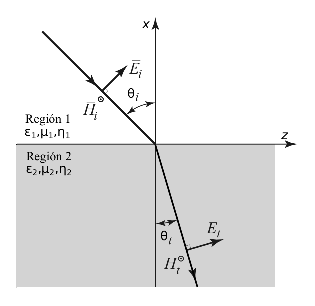
\includegraphics[width=0.5\textwidth]{intro_electro/onda-superficie-incidencia-brewster.eps}
	\caption{Ilustración del comportamiento de una onda plana durante la incidencia con ángulo de Brewster.}
	\label{fig:onda-superficie-brewster}
\end{figure}

\begin{subequations}
	\label{eq:ondas-superficie-campos}
	\begin{align}
	{H_1}_y &= A e^{-j\ (z\; \overbrace{k_0\;sin \theta_i}^{\beta} - x\; \overbrace{k_0\;cos \theta_i)}^{h_1}},\;\; x>0 & j\omega\epsilon E_x &= -\frac{\partial H_y}{\partial z} \\
	{H_2}_y &= A T e^{-j\; (z\; \overbrace{k\; sin \theta_t}^{\beta} - x\; \overbrace{k\; cos \theta_t)}^{h_2}},\;\; x<0   & j\omega\epsilon E_z &= -\frac{\partial H_y}{\partial x} 
	\end{align}
\end{subequations}

Expresando los campos a uno y otro lado del plano, en función del sistema de coordenadas de la figura \ref{fig:onda-superficie-brewster}, se obtienen, en forma general, las expresiones mostradas en la ecuación \ref{eq:ondas-superficie-campos}. La componente longitudinal de los vectores de onda es igual a ambos lados de la interfaz, de modo que es $k \; \sin \; \theta_t = \beta = k_0 \; \sin \; \theta_i$. Las componentes normales a la interfaz, que llamaremos $h_i$, $i=1,2$, deben cumplir que

\begin{align}
& h_1^2 + \beta^2 = k_0^2 &h_2^2 + \beta^2 = k^2
\end{align}

Las impedancias de onda en ambas regiones es la relación entre los campos tangenciales a la interfaz sobre la que se incide, de modo que:

\begin{subequations}
\label{eq:impedancia-onda-superficie}
\begin{align}
	Z_1 = \frac{{E_z}_1}{{H_y}_1} = \eta_0 \; cos\; \theta_i \implies Z_1 = \frac{h_1}{k_0} \eta_0 \label{eq:impedancia-onda-incidente-onda-sup}\\
	Z_2 = \frac{{E_z}_2}{{H_y}_2} = \eta \; cos \; \theta_t \implies Z_2 = \frac{h_2}{k} \eta \label{eq:impedancia-onda-transmitida-onda-sup}
\end{align}
\end{subequations}

Para poder considerar que toda la energía de la onda incidente se transmite a la interfaz, $Z_1 = Z_2$, de modo que, igualando las ecuaciones \ref{eq:impedancia-onda-incidente-onda-sup} y \ref{eq:impedancia-onda-transmitida-onda-sup}, recordando que $k = \omega \sqrt{\mu \epsilon}$, igualando las componentes de $\vec{k}$ paralelas a la interfaz y asumiendo que $\mu_2 = \mu_0$, queda expresada la siguiente relación, que ilustra el caracter complejo de las componentes normales a la interfaz, $h_1$ y $h_2$:

\begin{equation}
	h_1\; (\epsilon' - j \epsilon'') = \epsilon_0 h_2
\end{equation}

De esta manera, $h_1 = h_1' - jh_1''$ y $h_2 = h_2' + jh_2''$. Como $k_0^2 = \beta^2 + h_1^2$, entonces $\beta = \beta' - j \beta''$ posee también un valor complejo.

Si se considera una superficie con una impedancia de onda normalizada respecto de $\eta_0$, $Z_s = R_s + j X_s$, independiente del ángulo de incidencia, para polarización TM, entonces en base a la ecuación \ref{eq:impedancia-onda-incidente-onda-sup}, resulta:

\begin{align}
	h &= h'+jh'' = k_0 \frac{Z_1}{Z_0} = k_0 Z_s = k_0 R_s + j k_0 X_s \implies \\
	\beta &= \beta' - j\beta'' = \sqrt{(k_0^2 - h^2)} = \sqrt{k_0^2 - (k_0 R_s + j k_0 X_s )^2} \nonumber\\
		&= k_0 \sqrt{1+X_s^2 - R_s^2 - 2jR_s X_s} 
\end{align}

Reemplazando el valor de $h$ en la expresión del campo magnético de la ecuación \ref{eq:ondas-superficie-campos}, se observa que el campo presenta un decrecimiento exponencial en la dirección normal a la superficie si el valor de $X_s$ es positivo, de manera que presente una reactancia inductiva, que además debe ser grande para que la onda de superficie se mantenga cercana a la superficie. Si, además, el valor de $R_s$ es lo suficientemente pequeño, $\beta''$ será pequeño y habrá baja atenuación en la dirección de propagación.

La velocidad de propagación se obtiene directamente de la componente real de $\beta$ que, si $R_s$ es pequeño y $X_s$ es grande, resulta: $\beta' = k_0 \sqrt{1+X_s^2}$, dando lugar a que la velocidad de propagación sobre la superficie resulte: $v_p = \omega/\beta' = c / \sqrt{1+X_s^2}$. En los casos en que la componente reactiva de la impedancia de superficie es grande, el valor de la velocidad de propagación es menor al de la luz.

En el caso de una interfaz aire-conductor, la componente inductiva de la impedancia de superficie resulta igual a la componente resistiva, de forma que $\eta = (1+j)/(\sigma \delta)$ \cite{Fernandez:Electromag}. Aplicando las ecuaciones \ref{eq:impedancia-onda-superficie}, se obtiene que

\begin{align}
	h &= k_0 (1+j) \sqrt{\frac{k_0}{2 \sigma Z_0}} \\
	\beta &= k_0 \sqrt{1-\frac{j k_0}{\sigma Z_0}} \approx k_0 - \frac{j k_0^2}{2 \sigma Z_0}
\end{align}

En general, un plano conductor soporta ondas de superficie, pero no es capaz de lograr una atenuación en la dirección normal al mismo tal que la energía se mantenga concentrada en la superficie para poder ser utilizada como guía de ondas. Para lograr que la energía de la onda decaiga rápidamente lejos de la interfaz es necesario aumentar considerablemente la resisitividad de la superficie, para lo que se suele agregar al conductor una capa dieléctrica.
\subsection{Línea microstrip}

\section{Resonadores}

\section{Líneas de transmisión}
\label{subsec_lineas_de_transmision}
%%%%
LOREM IPSUM
% Venkateswaran, cap 1.
%%%%
\section{Antenas}
\label{subsec_antenas}
%%%%
LOREM IPSUM
%%%%
\subsection{Regiones de campo}
\label{subsubsec_regiones_de_campo}
%%%%
LOREM IPSUM
%%%%
\subsection{Diagramas de radiación}
\label{subsubsec_diag_de_rad}
%%%%
LOREM IPSUM
%%%%
\subsection{Potencia total radiada e intensidad de radiación}
\label{subsubsec_pot_total_radiada}
%%%%
LOREM IPSUM
%%%%
\subsection{Directividad, eficiencia y ganancia}
\label{subsubsec_directividad}
%%%%
LOREM IPSUM
%%%%
\subsection{Polarización}
\label{subsubsec_polarizacion}
%%%%
LOREM IPSUM
%%%%

\subsection{Impedancia de entrada}
\label{subsec_imp_entrada}
%%%%
LOREM IPSUM
%%%%
\subsection{Acoplamiento mutuo}
\label{subsec_acoplamiento}
%%%%
LOREM IPSUM
%%%%
\subsection{Dieléctricos y pérdidas dieléctricas}
\label{subsec_dielectricos}
%%%%
LOREM IPSUM
% LibroSinNombre, pagina 816
%%%%
\subsection{Parámetros S}
\label{subsec_parametros_s}
%%%%
LOREM IPSUM
% Pozar, pag 178
%%%%

\subsection{Antenas Microstrip}
\label{subsec_antenas_microstrip}
%%%%
LOREM IPSUM
%%%%
\subsubsection{Modelo de líneas de transmisión}
\label{subsubsec_microstrip_modeloLineas}
%%%%
LOREM IPSUM
% LibroSinNombre, pahgina 534
%%%%
\subsubsection{Modelo de cavidades multimodo}
\label{subsubsec_microstrip_modeloCavidades}
%%%%
LOREM IPSUM
% Pozar, rezonadores, capitulo 6
%%%%

\subsection{Acoplamiento mutuo en antenas Microstrip}
\label{subsec_acoplamiento_microstrip}
%%%%
LOREM IPSUM
%%%%
% LibroSinNombre, pagina 562 y 631
\subsubsection{Ondas de superficie}
\label{subsubsec_microstrip_ondas_superficie}
%%%%
LOREM IPSUM
%%%%
% Engheta, pagina 289
% Rahim (tesis), pagina 28
% Collin, capitulo de Surface waveguides, pag 697
% Paper de Barlow.
% Pozar, pag 138
% Tesis de Kovacs, pagina 8
% Tesis de Zheng, apendice A, pag 48. Interfaces con diel y con metales.

